%% ------------------------------------------------------------------------- %%
\chapter{Introdução}
\label{cap:introducao}

O avanço e descoberta de novas tecnologias faz parte da história da humanidade. Em economia cunha-se o termo \textit{General Pupose Technology}, que são avanços tecnológicos que afetam toda uma economia. Entre estes avanços tecnológicos temos o motor a vapor, posteriormente substituído pelo motor a combustão interna. O computador representou um avanço tecnológico. A internet representou um grande salto na maneira como são feitas as comunicações e transações financeiras hoje. E atualmente, inteligência artificial está caminhando para romper esta barreira e impactar toda a economia \todo{adicionar referências}.

As primeiras redes neurais foram concebidas em 1945, o famoso perceptron. Mas desde 1945 e até os dias atuais, a área de inteligência artificial passou por vários momentos. Dentre eles momentos de euforia, no qual pesquisadores e entusiastas já previam rôbos substituindo o ser humano e que todas as tarefas seriam feitas pelos computadores. E momentos de pouco investimento, chamado \textit{AI Winter}, devido as muitas expectativas e poucos resultados. Porém demorou pelo menos 50 anos para termos os primeiros indícios do potencial desta área. Inteligência artificial abrange várias áreas. E a área que mais se destaca atualmente é a área de aprendizagem de máquina. Mais especificamente aprendizagem de máquina profunda. \todo{corrigir este parágrafo. Adicionar datas certas}

Alan Turing após conceber o primeiro computador em 1930 (ver data e se está correto), disse que o computador poderia resolver qualquer problema desde que fosse possível passar as regras. O computador resolve facilmente operações aritméticas e até mesmo consegue ganhar de um campeão mundial de xadrez (1997). Porém, tarefas que são simples para o ser humano como reconhecer faces, falas ou traduzir textos, são tarefas muito complexas para o computador, pois o ser humano não consegue traduzir estas ações em regras ou fórmulas para o computador. \todo{corrigir}

Porém, estes desafios de reconhecimento de imagens e tradução de textos foram superados pela máquina em 2015. Uma competição ImageNET no qual vários pesquisadores competem entre si para reconhecer milhares de imagem do banco imagenet. Um grupo do canadá apresentou o CNN, uma rede neural convolucional profunda no qual obteve 70\% de acurácia.

No ano posterior, ele obteve 97\%. Este desafio foi dado como superado. Não foi somente reconhecimento de imagens que o computador igualou e superou o ser humano. A IBM desenvolveu um computador que ganhou do ser humano no \textit{Jeopardy}. O Google desenvolveu o \textit{Alpha Go} que superou o campeão mundial de Go.

Todas estas conquistas feitas por pesquisadores e especialistas da área de inteligência artificial, foram feitas utilizando redes neurais profundas, mais especificamente redes neurais convolucionais e recorrentes. Tanto as redes convolucionais e redes recorrentes já eram conhecidas desde a década de 90. Com algumas exceções e outros detalhes, a maioria dos algoritmos já haviam sido desenvolvidas na década de 80 e 90. Porém só em 2015 o primeiro resultado veio a tona.

Neste período de 20 a 30 anos, ocorreram evoluções em outras áreas da computação que permitiu o salto em aprendizagem de máquina. Os principais fatores que contribuíram foram:

\begin{itemize}
    \item Aumento do processamento de CPU e GPU. Temos também pesquisas avançando em processadores específicos para a área de inteligência artificial como os TPUs
    \item Aumento da capacidade de armazenagem
    \item Acesso e democratização da internet, que permitiu gerar um grande volume de dados
    \item Avanços na pesquisa e no uso de arquiteturas de redes neurais mais eficientes para determinados tipos de problemas
\end{itemize}

Há outros fatores, mas estes fatores foram cruciais para o advento e o salto da aprendizagem de máquina atual. E atualmente cada vez mais empresas e governos estão investindo dinheiro na área de inteligência artificial. Há demandas para uso na área agrícola, investimentos, saúde, comércio. Empresas como o Google, IBM, Facebook, Apple e Amazon estão investindo bilhões de dólares nesta área. E uma das áreas que de aprendizagem de máquina é o processamento de linguagem natural. 

A área de processamento de linguagem natural pesquisa e trabalha com diversos problemas. Entre eles temos a tradução de textos, geração de textos \todo{verificar as areas de NLP} e um problema bastante comum é a solução de perguntas e respostas. O problema da pergunta e respostas consiste basicamente em dado uma pergunta e um conjunto de possíveis respostas, o algoritmo deve selecionar qual ou quais respostas respondem aquela pergunta.

Normalmente este problema consiste em perguntas e respostas de no máximo 1 parágrafo. É um desafio hoje criar modelos que dado uma pergunta, consiga responder com um artigo. Ou dado um livro ou artigo, responder perguntas a respeito \todo{adicionar referências}. Tanto que o próprio Google anunciou em janeiro de 2019, uma competição no qual deve-se criar um modelo capaz de responder ou não a perguntas, extraindo informação de artigos do Wikipedia. https://ai.googleblog.com/2019/01/natural-questions-new-corpus-and.html

A competição tem uma base aberta para os interessados. É possível conferir o ranking também das arquiteturas propostas pelos pesquisadores: https://ai.google.com/research/NaturalQuestions/leaderboard


A partir de uma base de conhecimento, FAQ, empresas e governos podem utilizar um modelo treinado neste contexto para responder perguntas e dúvidas de usuários. Ao fazer pesquisa no \textit{Google}, ele exibe perguntas e respostas sobre determinados tópicos pertinentes ao assunto buscado. Normalmente referem-se a dúvidas comuns de usuários. Exemplo está na figura \ref{fig:busca-google}.

\begin{figure}[h]
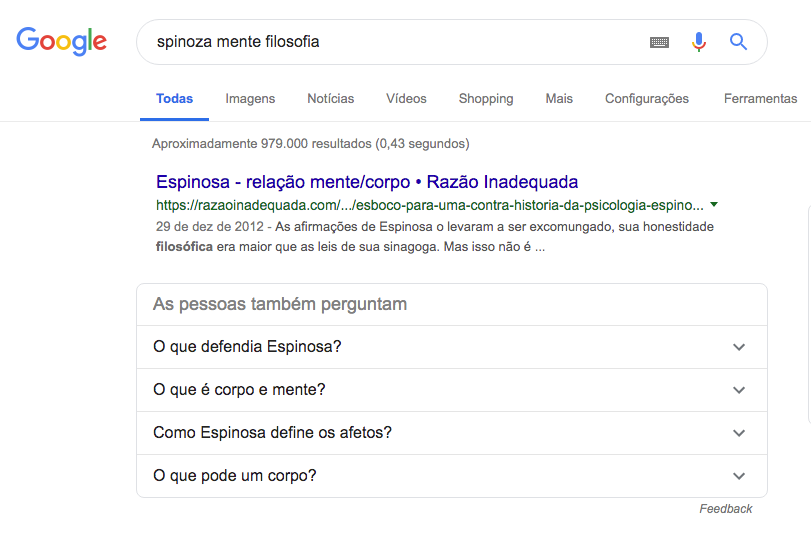
\includegraphics[width=12cm]{src/figuras/cap-introducao/busca-google-pergunta-resposta.png}
\caption{Perguntas relacionadas a pesquisa. Google and the Google logo are registered trademarks of Google LLC, used with permission.}
\label{fig:busca-google}
\end{figure}

Este problema de perguntas e respostas consiste em criar um modelo capaz de responder a dúvidas de usuários. A maioria das pesquisas atuais trabalham com linguagens naturais. Então, o usuário faz uma pergunta numa linguagem natural e o modelo responde com um texto em linguagem natural. Um outro desafio é dado uma pergunta em linguagem natural, criar um modelo capaz de responder em linguagem estruturada como XML, código fonte de linguagens como Java e/ou Python.

Antes de obter o modelo, é necessário definir uma arquitetura em rede neural e ter os dados para treinar. Com relação a arquitetura, pode-se utilizar, inicialmente, alguma das diversas arquiteturas propostas para o problema de perguntas e respostas em linguagem natural. 

Já em relação aos dados para o treinamento do modelo, é necessário criar uma base de dados de perguntas em linguagem natural e respostas numa linguagem estruturada. Uma possível fonte para este problema são os fóruns de programação. Junto com a internet, nasceu os fóruns. E os fóruns de programação fazem parte do cotidiano de todo programador. Diariamente vários programadores fazem e respondem perguntas sobre programação. E o site mais famoso e utilizado atualmente para perguntar e responder dúvidas de programação é o \textit{StackOverFlow}. 

Neste site, o usuário publica uma pergunta sobre programação. A pergunta feita pode ser simples e de uma linha só como, por exemplo, \textit{como ordenar um vetor de números em Python} ou pode ser uma pergunta mais longa que remete a um problema ou erro. Por exemplo, o usuário pode publicar um trecho de um programa e perguntar o motivo dele não funcionar. Os usuários do fórum respondem com uma possível solução para a pergunta e/ou problema. Caso esta solução consiga resolver o problema, o usuário que criou a pergunta pode marcar esta resposta como aceita. Além disso, os usuários do site votam para as perguntas e respostas que eles julgaram mais relevantes. 

Desde 2014, as perguntas e respostas feitas no site \textit{StackOverFlow} estão disponíveis no site https://archive.org/details/stackexchange. Com estes dados disponíveis, várias pesquisas foram feitas \todo{Adicionar referências}. E uma delas é a pesquisa feita pelo \cite{yao-2018}, no qual foram extraídas as perguntas e as respectivas respostas. A diferença desta pesquisa em relação as outras é que foram extraídas perguntas que tivessem uma resposta curta e direta. As perguntas que mais se encaixam nisso são as perguntas do tipo \textit{How-to}. E as respostas também são curtas e diretas, e foram extraídas somente os códigos-fontes que respondiam a pergunta feito pelo usuário. Neste caso, foram extraídas os códigos-fontes das respostas aceitas pelo usuário que fez a pergunta. 

Ao final desta pesquisa uma base de dados contendo pares de perguntas e códigos-fontes foi criada. Esta base foi disponibilizada ao final de 2018 \cite{yao-2018}. \citeauthor{yao-2018} utilizou uma rede neural recorrente bidirecional, no qual conseguiu obter uma precisão de 80\% com uma acurácia e recall de 84\% e 87\%. Os próprios autores citam possíveis caminhos que podem ser explorados para melhorar estes números. E um deles é o uso de redes convolucionais que mostraram bons resultados na aprendizagem de representação de textos.

Neste sentido, o presente trabalho busca verificar o comportamento de uma arquitetura de redes neurais convolucionais combinada com uma rede recorrente no problema de pares de perguntas e códigos-fontes.


%% ------------------------------------------------------------------------- %%
\section{Considerações Preliminares}
\label{sec:consideracoes_preliminares}

Neste trabalho, a arquitetura proposta que é composta pela combinação de redes convolucionais combinada com redes recorrentes é uma adaptação da arquitetura proposta por \cite{feng-2015}. Esta arquitetura de rede neural mostrou bons estudos no problema de perguntas e respostas em linguagem natural. 

Inicialmente, serão utilizados os dados disponibilizados pelo \citeauthor{yao-2018}. E para os resultados preliminares, serão levados em consideração os pares de perguntas e códigos fontes apenas em Python. 

Para ter uma base de comparação, o resultado da arquitetura de redes neurais que combina rede convolucional e rede recorrente será comparado com os resultados de uma rede neural convolucional e outro somente rede neural recorrente.


%% ------------------------------------------------------------------------- %%
\section{Objetivos}
\label{sec:objetivo}

O objetivo do presente trabalho é avaliar o desempenho de uma arquitetura de rede neural composta por uma rede neural convolucional e rede neural recorrente num problema de pares de perguntas e códigos-fontes. Neste estudo, busca responder a seguinte pergunta:

\begin{itemize}
    \item Qual o desempenho de uma arquitetura de rede neural composta pela combinação de uma rede neural convolucional e rede neural recorrente no problema de pares de perguntas e códigos-fontes? 
\end{itemize}

Ao analisar o desempenho, o principal objetivo é saber se o modelo obtido através do treinamento nos dados do \textit{StackOverFlow} é capaz de aprender. E aprender, significa extrair o conhecimento dos dados disponibilizados no treinamento e ser capaz de generalizar. Caso o modelo consiga generalizar, há a possibilidade de aplicabilidade prática.

%% ------------------------------------------------------------------------- %%
\section{Contribuições}
\label{sec:contribucoes}

As principais contribuições deste trabalho são as seguintes:

\begin{itemize}
  \item Avaliação do desempenho da aplicação de uma arquitetura de rede neural composta pela combinação de redes neurais convolucionais e redes recorrentes no problema de pares de perguntas e códigos-fontes.
  \item Disponibilização do código fonte adaptado para uso futuro por outros pesquisadores e/ou interessados.
\end{itemize}

%% ------------------------------------------------------------------------- %%
\section{Organização do Trabalho}
\label{sec:organizacao_trabalho}

No Capítulo~\ref{cap:trabalhos-relacionados}, apresentamos os conceitos e trabalhos relacionados ao problema de perguntas e respostas em processamento de linguagem natural. No capítulo~\ref{cap:problema}, discutimos o problema de pesquisa proposto para o presente trabalho, a arquitetura proposta e apontamos detalhes dos dados utilizados pertinentes a pesquisa. 
No capítulo~\ref{cap:resultados-preliminares}, exibimos os resultados preliminares da arquitetura proposta utilizando os dados do \cite{yao-2018}. E também discutimos as principais dificuldades encontradas para adaptar a arquitetura do \cite{feng-2015} para resolver problema de pares de perguntas e códigos-fontes. Já no capítulo~\ref{cap:cronograma}, temos as considerações finais, proposta do cronograma e os próximos passos da pesquisa.
